\documentclass{beamer}

\usepackage{amssymb}
\usepackage[english]{babel}
\usepackage{graphicx}
\usepackage{physics}

\usetheme{Berlin}
\usecolortheme{beaver}
\setbeamertemplate{footline}[frame number]
\setbeamertemplate{itemize item}[circle]
\graphicspath{ {./img/} }

\title{2D Causal Dynamical Triangulations}
\subtitle{Using Markov-Chain Monte Carlo methods}
\author{T.B.H. Gerstel \and J.G.R. van der Duin}
\date{December 2021}
\institute{Radboud University Nijmegen}
\logo{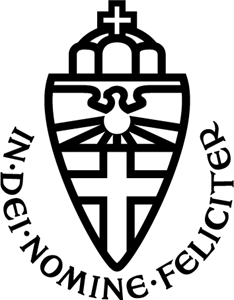
\includegraphics[height=1cm]{radboud}}

\begin{document}

\frame{\titlepage}

\begin{frame}
    \frametitle{Overview}
    \tableofcontents
\end{frame}

\section{Theory}

% Suggested topics:
% Maybe something about what makes CDT different from DT, how causality is implemented?

\begin{frame}
    \frametitle{Goal}
    Extract information from Quantum Gravity path integral:
    \begin{equation}
        Z = \int \mathcal{D}[g_{\mu \nu}] e^{i S[g_{\mu \nu}]}
    \end{equation}
    With Einstein-Hilbert action:
    \begin{equation}
        S[g_{\mu \nu}]
        =
        \frac{1}{16 \pi G}
        \int_\mathcal{M} \dd[4]{x} \sqrt{-g}
        (R(x) - 2 \Lambda)
    \end{equation}
    Problem: How can we integrate over geometries? \\
    Solution: Triangulations!
\end{frame}

\begin{frame}
    \frametitle{Causal Dynamical Triangulations}
    \begin{columns}
        \begin{column}{0.7\textwidth}
            Create causal structure:
            \begin{itemize}
                \item In (1 + 1)D: use triangles
                \item Timeslice: ring of $L$ links
                \item Universe: sequence of $T$ timeslices connected by triangles
            \end{itemize}
            Example: $T = 3$, $L = 5$, $N = 2TL = 30$
        \end{column}
        \begin{column}{0.3\textwidth}
            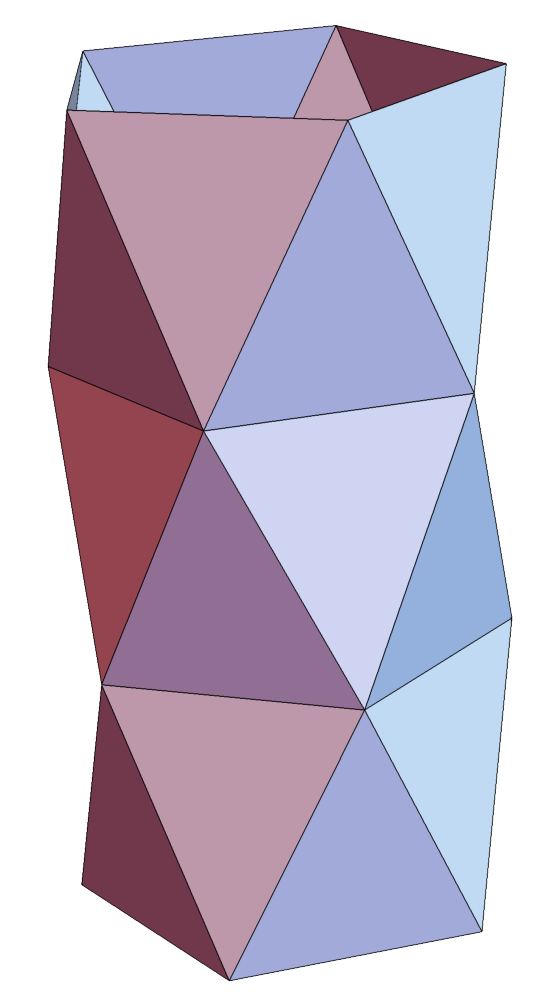
\includegraphics[width=1\textwidth]{uniform}
        \end{column}
    \end{columns}
\end{frame}

\begin{frame}
    \frametitle{Technicalities}
    Some technicalities:
    \begin{itemize}
        \item In 2D: constant curvature
        \item Action proportional to volume ($N_2$)
        \item Wick rotation
        \item Label triangles
    \end{itemize}
    Resulting partition function:
    \begin{equation}
        Z_\ell = \sum _{T_\ell} \frac{1}{N_2(T_\ell)!} e^{-\lambda N_2(T)}
    \end{equation}
\end{frame}

\section{Model}

\begin{frame}
    \frametitle{Volume fixing}
    Split $Z$ into fixed volume contributions:
    \begin{equation}
        Z
        =
        \sum_{T_\ell} \frac{1}{N_2(T_\ell)!} e^{-\lambda N_2(T_\ell)}
        =
        \sum_{n = 0}^\infty \Omega(n) \frac{e^{-\lambda n}}{n!}
    \end{equation}
    It turns out that $\Omega(n) \sim n! 2^n$ \\
    Problem:
    \begin{itemize}
        \item $\lambda > \ln 2$: typical triangulation has a very small volume $\to$ cannot extract useful data
        \item $\lambda < \ln 2$: triangulation keeps growing $\to$ equilibrium cannot be reached
    \end{itemize}
    Our solution: fix the number of triangles $N_2$ \\
    Futher advantage: distribution becomes uniform
\end{frame}

\begin{frame}
    \frametitle{Volume fixing (2)}
    How can we implement this volume fixing? \\
    Possible solution: add a constraint term $\delta S = \epsilon \abs{N_2(T) - n}$ \\
    Issues:
    \begin{itemize}
        \item Introduces an extra parameter $\epsilon$
        \item Results in more rejections
    \end{itemize}
    Our solution: use update rules that preserve $N_2$
\end{frame}

\section{Implementation} % Maybe do switch somewhere in this section?
\begin{frame}
    \frametitle{Observables}
    
    % To be able to analyse the behaviour of the model, meaningful observables need to be found
    \begin{itemize}
        \item Difficult to find meaningful observables
        \item Cannot depend on labeling $\rightarrow$ average over geometry
        \item ...
    \end{itemize}
    \begin{figure}
        \centering
        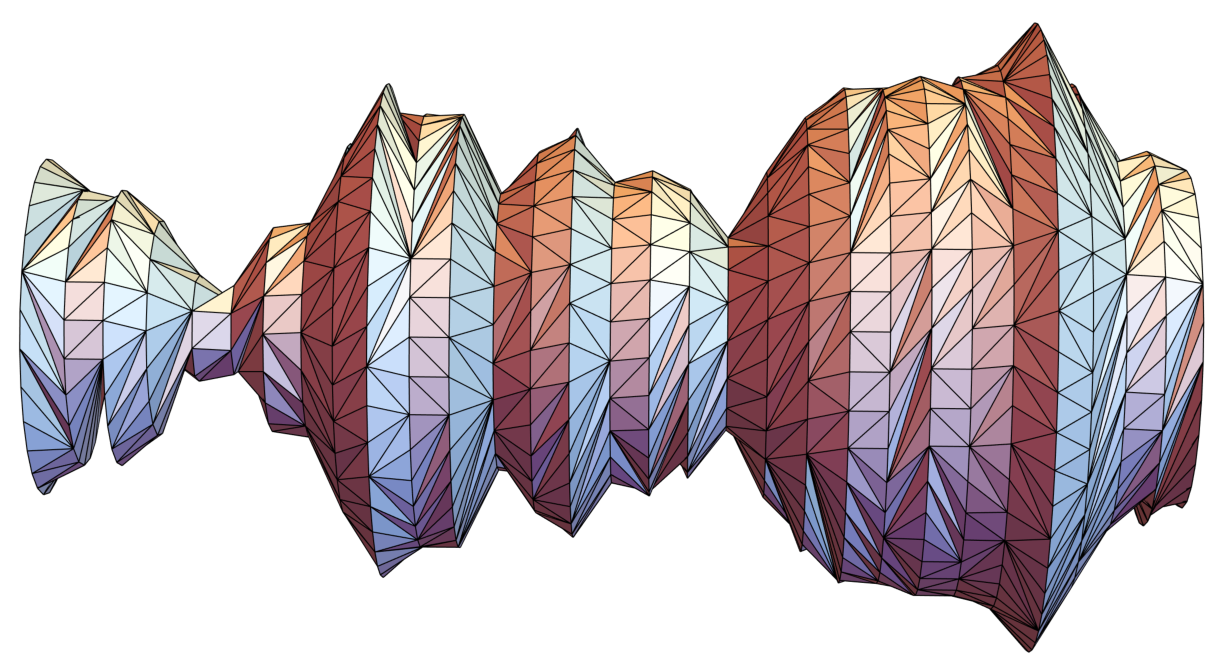
\includegraphics[width=0.6\linewidth]{img/triangulation.pdf}    
    \end{figure}
    
\end{frame}

\section{Data Analysis}
% Saving data, determining equilibirum and correlation

% In practice chose to write the entire length profile to disk to be able to later decide on specific observable, the disk space is still minimal
% In the end we wish to look at the behaviour of the autocorrelation of the length profile for large N, but we have not yet done so
% For simiplicity we have as of yet only look at the behaviour of the std
% We wish to obtain the behaviour of std for large N, for this we wish to use batching to be able to make good estimates of the error
% For this we need estimates of the equilibrium time, to make sure the system is thermalized; and estimates of the correlation time to reduce the amount of data that needs to be saved and to know how big to take the batches

% It is difficult to construct another initial state so we , so to estimate the equilibrium time we use ...
% And we notice the equilibirum time is rather small and constant for different N (in terms of sweeps), because our initial state is very close to equilibirum.

% We have a single model parameter which can still be tuned, so we can tune it to make the correlation time minimal.
% We determine the correlation time be simulation long traces of the std and looking for 'exponential decay' behaviour in the autocorrelation of the std with respect to the simulation step time.
% Determining this for different ratios we see there is a large minimum around 0.4, and notice the correlation time is not very sensitive around this minimum; so it should be save to choose 0.4
% We perform similar measurements for different L values, which shows the correlation time is roughly constant; and we look for different T values which suggests tcor grows roughly with O(T).
% Thus in total we find that tcor grows with O(N) in sweeps thus O(N^2) in MC steps, which is very unfortunate as this inhibits us from performing large simulations. But what we can do is keep T constant and make N large

% First results show that std gros as a non-trivial power in N

\section{Outlook}
% Tying it all together and explain what we still expect to do
\begin{frame}
    \frametitle{Outlook}
    \begin{itemize}
        \item Look at \emph{autocorrelation}
        \item Find collapse of \emph{autocorrelation}
    \end{itemize}
    \begin{figure}
        \centering
        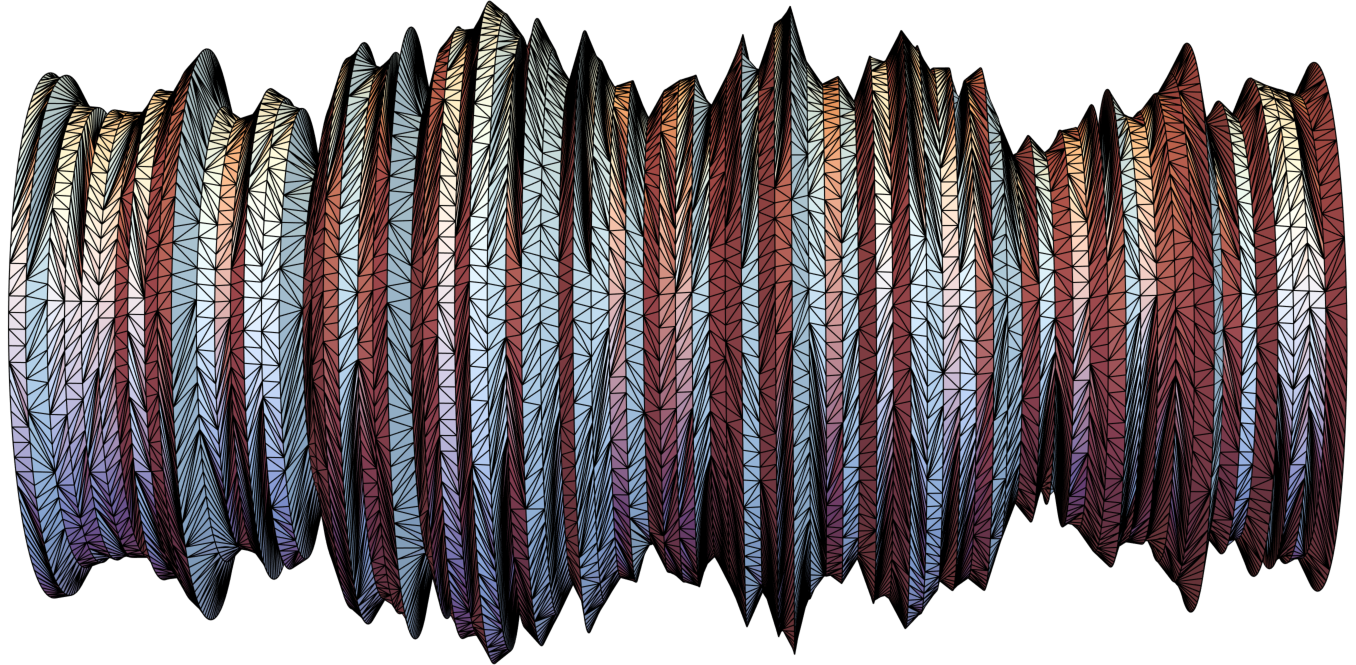
\includegraphics[width=0.9\linewidth]{triangulation_large.pdf}
    \end{figure}
\end{frame}


\end{document}